\section{Analysis}
In this section we obtain the analytical first order theory for orbits about the satellite and discuss the implications. For this we will double-average the disturbing function, obtain the equivalent Lagrange Planetary Equations, and analyze their implications for the case of a low altitude orbiter at high inclination scientific orbits.

\subsection{Averaging the disturbing function}
In averaging the disturbing function for the tidal perturbation, we consider that the effect of the tidal perturbation for a single orbit small so it can be approximated by keeping all orbital elements constant.
\begin{equation}
\tilde{\mathcal{R}}_P = \frac{1}{2\pi} \int_0^{2\pi} \mathcal{R}_P dM =\frac{1}{2}(-r^2 + 3 x^2)
\end{equation}

This averaging can be done in either true or eccentric anomaly. The first option involves expanding $r$ as Fourier cosines series for which only the constant and second harmonics don't vanish after integration. Eccentric anomaly is more involved but more straight forward so we will use it, we have to change the integration variable to $E$, and using the appropriate expressions for $x$ and $r$ and expanding into harmonics of $E$ it is clear that only the constant term will survive. 
\begin{align}
r &= a (1 - e \cos E) \\
dM &= \frac{r}{a} dE = (1 - e \cos E) dE
\end{align}

$x$ is expressed the rotating frame coordinates, which rotate with angular velocity $1$. We define the longitude of the ascending node $\lambda$ as a time varying constant, even in the osculating orbit, that references the ascending node in satellite coordinates (the satellite rotates synchronously with the reference frame). Then $x$ can be obtained by a rotation from the perifocal coordinates $\xi, \eta$, functions of the orbital parameters $a,e$, using the instantaneous orbital parameters $\lambda, i, \omega$.
\begin{equation}
\begin{aligned}
x =& (-\cos\lambda \cos\omega + \cos i \sin\lambda \sin\omega) \xi \\
&+ (\cos i \cos\omega \sin\lambda + \cos\lambda \sin\omega) \eta \\
=& a (-\cos\lambda \cos\omega + \cos i \sin\lambda \sin\omega) (1 - e \cos E) \\
&+ a \sqrt{1-e^2} (\cos i \cos\omega \sin\lambda + \cos\lambda \sin\omega) \sin E
\end{aligned}
\end{equation}

To obtain after the integration:
\begin{equation}
\begin{aligned}
\tilde{\mathcal{R}}_P &= \frac{1}{64} a^2 \left[15 e^2 \cos 2 \omega  \left(2 \cos 2i + 6 \cos 2 \lambda +4 \sin^2 i \right) \right.\\
&\left. -120 e^2 \cos i \sin 2 \lambda \sin 2 \omega + 2 \left(3 e^2+2\right) \left(6 \sin^2 i \cos 2 \lambda +3 \cos 2i +1\right) \right]
\end{aligned}
\end{equation}

We now introduce the second averaging assumption. If we consider the mean motion of the orbiter about the satellite to be $n \gg 1$, an assumption that will hold in most scenarios in the solar system, then the orbiter will complete many revolutions about the satellite while completing one about the planet. If these perturbations for a single planetary orbit are small enough, we can again average the effect of $\lambda$ which as we stated, incorporates the rotation about the planet to obtain $\bar{\mathcal{R}}_P$:
\begin{equation}
\bar{\mathcal{R}}_P = \frac{1}{2\pi} \int_0^{2\pi} \tilde{\mathcal{R}}_P d\lambda = \frac{1}{32} a^2 \left[30 e^2 \sin^2 i \cos 2 \omega +\left(3 e^2+2\right) (3 \cos 2i +1)\right]
\end{equation}

Following the same process we obtain the disturbing function for one revolution. There's no need to consider the second averaging about the planet for the perturbation due to the oblateness $\bar{\mathcal{R}}_2$ since it would only average out the $J_{21}, J_{22}$ terms which have been disregarded beforehand. For the sake of simplicity we refer to the class notes where an equivalent expression for  the averaging of the $J_2$ perturbation was found:
\begin{equation}
\bar{\mathcal{R}}_2 = \frac{n^2 J_2}{8 (1-e^2)^{3/2}} \left(1 + 3 \cos 2i\right)
\end{equation}

The global averaged disturbing function $\bar{\mathcal{R}}$ is found as the sum of $\bar{\mathcal{R}}_P$ and $\bar{\mathcal{R}}_2$.

\subsection{Derivation of the Lagrange Planetary Equations}
For the derivation of the Lagrange Planetary Equations, we leverage the linearity of the perturbation function. We will consider the contributions of the perturbing function due to tidal force and those due to the oblateness separately, and we will simplify them using the same assumptions. Then we will find the total rate of change as the sum of those.

The Lagrange Planetary equations considering only the tidal perturbation are:
\begin{align}
\dot{a} &= 0\\
\dot{e} &= \frac{15}{8} \frac{e \sqrt{1-e^2}}{n} \sin^2 i \sin 2\omega \\
\dot{\lambda} &=-1 - \frac{3}{8} \frac{2 + 3 e^2 -5 e^2 \cos 2 \omega }{\sqrt{1-e^2} n} \cos i \\
\frac{di}{dt} &= -\frac{15}{16} \frac{e^2 }{\sqrt{1-e^2} n} \sin 2i \sin 2\omega\\
\dot{\omega} &= \frac{3}{16} \frac{3 +10 \cos 2i \sin^2 \omega + \left(5-10 e^2\right) \cos 2 \omega +2 e^2}{\sqrt{1-e^2} n} \\
\dot{M} &= n-\frac{3}{16} \frac{\left(e^2+1\right) \sin ^2(i) \cos (2 \omega )+3 \left(3 e^2+7\right) \cos (2 i)+3 e^2+7}{n}
\end{align}

And the equations for the $J_2$ perturbations are:
\begin{align}
\dot{a} &= 0\\
\dot{e} &= 0\\
\dot{\lambda} &=- 1+ \frac{3}{2} \frac{n J_2}{a^2 \left(1-e^2\right)^2} \cos i \\
\frac{di}{dt} &= 0\\
\dot{\omega} &= -\frac{3}{8} \frac{n J_2 (3 + 5 \cos 2i)}{a^2 \left(1-e^2\right)^2} \\
\dot{M} &= n \left[1 + \frac{3}{8} \frac{J_2}{a^2} \left( 1+ 3 \cos 2i\right) \right]
\end{align}

Since we have averaged the perturbing function with respect to one revolution around the satellite and the planet both $M$ and $\lambda$ are ignorable coordinates whose averaged contribution is already included the equations above. Thus for the analysis of the shape of the orbit we can disregard the equations for both the mean motion and the node.

Instead of combining the equations above directly, we first consider the extra assumptions that we can introduce for the case of the low altitude orbiter.

\subsection{Simplifying the equations for a low altitude orbiter}
Our interest lies in the behavior of the orbits for a low altitude orbiter. In this case the eccentricity must be small since the radius of the satellite will limit the periapsis. 

Then the equations above can be simplified by keeping only the terms up to the first power of $e$. The equations considering the tidal and oblateness perturbations are:
\begin{align}
\dot{a} &= 0\\
\dot{e} &= \frac{15}{8} \frac{1}{n} e \sin^2 i \sin 2\omega\\
\frac{di}{dt} &= 0\\
\dot{\omega} &= \frac{3}{8} \frac{1}{n}\left[4 - \sin^2 i+ 5 \sin^2 i \cos 2\omega \right] -\frac{3}{4} \frac{n J_2 }{a^2} \left(4 - 5 \sin^2 i\right)
\end{align}

Where we have used trigonometric identities to make the expressions for $\dot{e}$ and $\dot{\omega}$ more similar.

For the first order approximation for small $e$ we observe that the inclination and the semi-major axis stay constant. The behavior of the orbit can be reduced to the motion of the eccentricity in the orbital plane. Therefore we have successfully reduced the behavior of the orbit to a two-dimensional problem for which $a$ and $i$ are parameters.

\subsection{The motion of the eccentricity vector}
In Scheeres \cite{scheeres2001stability} an analytical solution is provided for the equations above. However, here we deem more insightful to examine the properties of the behavior in terms of the phase space and the properties of conservative dynamical systems.

We define the following variable changes to further simplify the equations of motion:
\begin{align}
\chi &= \frac{n^2}{a^2} J_2 = \frac{J_2}{a^5}  \\
\alpha &= (1+ 2\chi) \frac{4 - 5 \sin^2 i}{5 sin^2 i} \\
\kappa &= \frac{15}{8} \frac{1}{n} \sin^2 i
\end{align}

And we introduce the independent variable $\tau = \kappa t$ which is just a scaling of the time that simplifies the equations. Using these, we obtain the equations of motion:
\begin{align}
\frac{de}{d\tau} &= \sin 2\omega \ e \\
\label{domegadtau}
\frac{d\omega}{d\tau} &= \cos 2\omega+ \alpha
\end{align}

This is a nonlinear system of equations. The second equation in $\omega$ is decoupled from the equation of $e$. The behavior of the argument of the periapsis depends on $\alpha$, for $\alpha^2>1$ the change rate in $\omega$ will be monotonic, for $\alpha^2<1$ there will be several equilibria solutions (for the argument of periapsis only, not the eccentricity vector), with some being stable and others unstable. The behavior of $e$ in instantaneously exponential with gain $\sin 2\omega$ in the eccentricity module so it will depend on the behavior of the argument of periapsis. 

The only possible equilibrium for the this system is with $e=0$ for any $\alpha$ or for the case of $\alpha^2=1$, but this is not a desirable operating point since the system may change properties as discussed above. While a linearized analysis of the equations may give some insight on the local equilibrium properties it does not offer insight on the global behavior. A similar problems arises for the analytic solution, it does not offer extra insight in understanding the stability properties of the system. Probably the most insightful approach is to leverage that the system is conservative and has a unique equilibrium point, then due to the symplectic properties of hamiltonian systems \cite{scheeres2012orbital55} \cite{meirovitch1970methods}, the equilibrium will be either a not asymptotic but stable point, in other words it will have a stable and unstable manifold. In fact, the $\alpha^2=1$ is a bifurcation for the system.

In figure \ref{fig:eccentricityPhasePortraitStable} we reproduce the phase plane for the eccentricity vector in polar coordinates for the case of $\alpha^2>1$, the eccentricity vector exhibits a periodic motion which is stable. In figure \ref{fig:eccentricityPhasePortraitStable} we display the case for $\alpha^2<1$ and we can clearly observe that the global behavior is unstable with an attractive mode and a unstable mode. Beside, the determining the stability behavior of the system, $\alpha$ also determines the positions of the stable and unstable manifolds since they satisfy equation \ref{domegadtau}.

\begin{figure}[h]
	\centering
	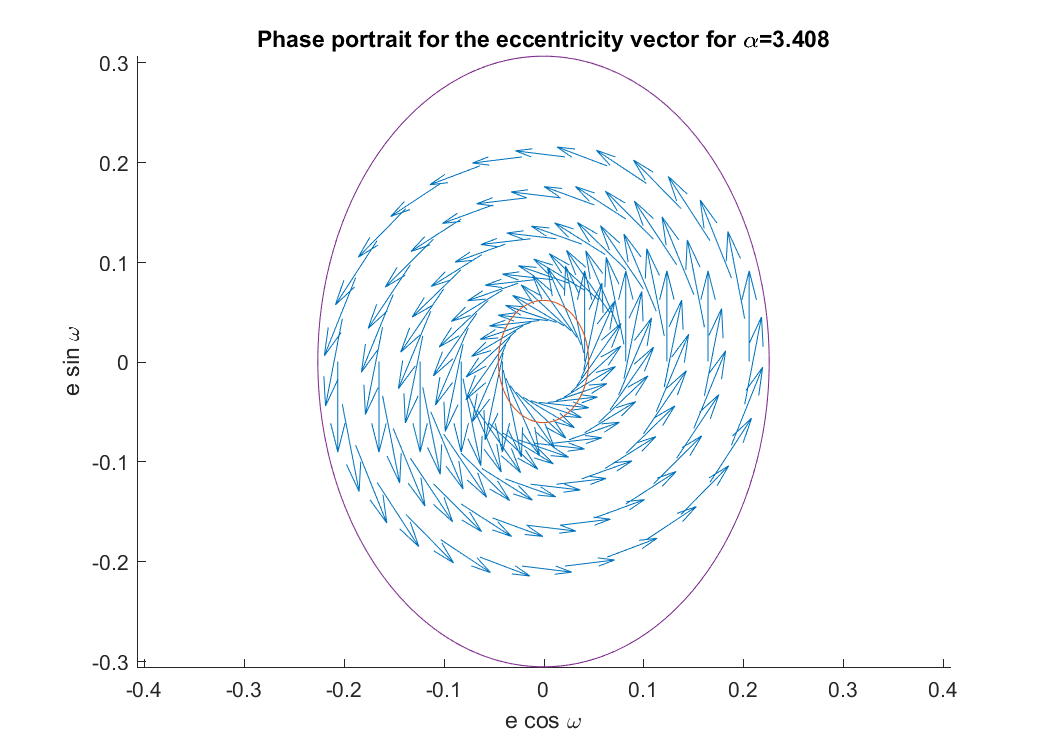
\includegraphics[height=2.5in]
	{figures/Europe400km01e30i/EccentricityPhasePortrait.png}
	\caption{Phase portrait for the eccentricity vector in a stable configuration: $\chi = .2746, \alpha = 3.4080$}
	\label{fig:eccentricityPhasePortraitStable}
\end{figure}

\begin{figure}[h]
	\centering
	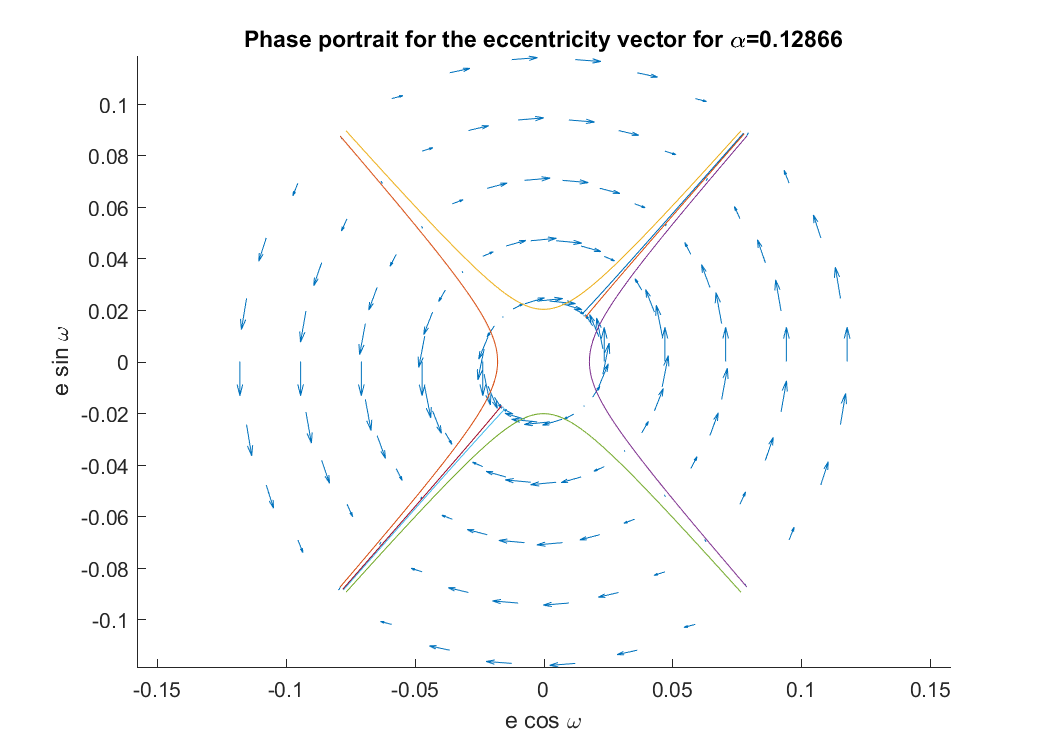
\includegraphics[height=2.5in]
	{figures/Europa200km01e60i/EccentricityPhasePortrait.png}
	\caption{Phase portrait for the eccentricity vector in a unstable configuration: $\chi = 0.4650, \alpha = 0.1287$}
	\label{fig:eccentricityPhasePortraitUnstable}
\end{figure}

The existence of the attractive mode could be used to circularize an orbit, which is the approach followed by JUICE \cite{esa2014juice}. It is important to note that these equations are an averaged first order approximation of a more complex system, this means that even if there is an attractive mode that could be exploited to circularize the orbit, there will inaccuracies that will excite the unstable modes so the control action required to stay on the attractive manifold may be significant.

Finally, we discuss the kind of orbits that will lead to both behaviors. From the definitions of $\chi$ and $\alpha$ we can observe that the involved parameters are on, one the one hand the inclination of the orbit $i$, and on the other the semi=major axis of the orbiter $a$ and the $J_2$ harmonic. The dominant factor is the inclination, low inclination orbits will lead to bigger $\alpha$ and therefore stability, high inclination orbits will tend to be unstable, effect that will be increased if the effect the oblateness of the planet as measured by $\chi$ increases. At the same time the semi-major axis $a$ and inclination $i$ are present in the time scale $\kappa$, meaning that for high inclination and high altitude orbits the effect in the eccentricity will be slower.

Since we are considering the application of this theory to scientific orbiters, inclinations will typically be high and we will expect the unstable behavior.